\begin{figure}[htbp]
  \centering

  \begin{subfigure}[t]{0.48\textwidth}
    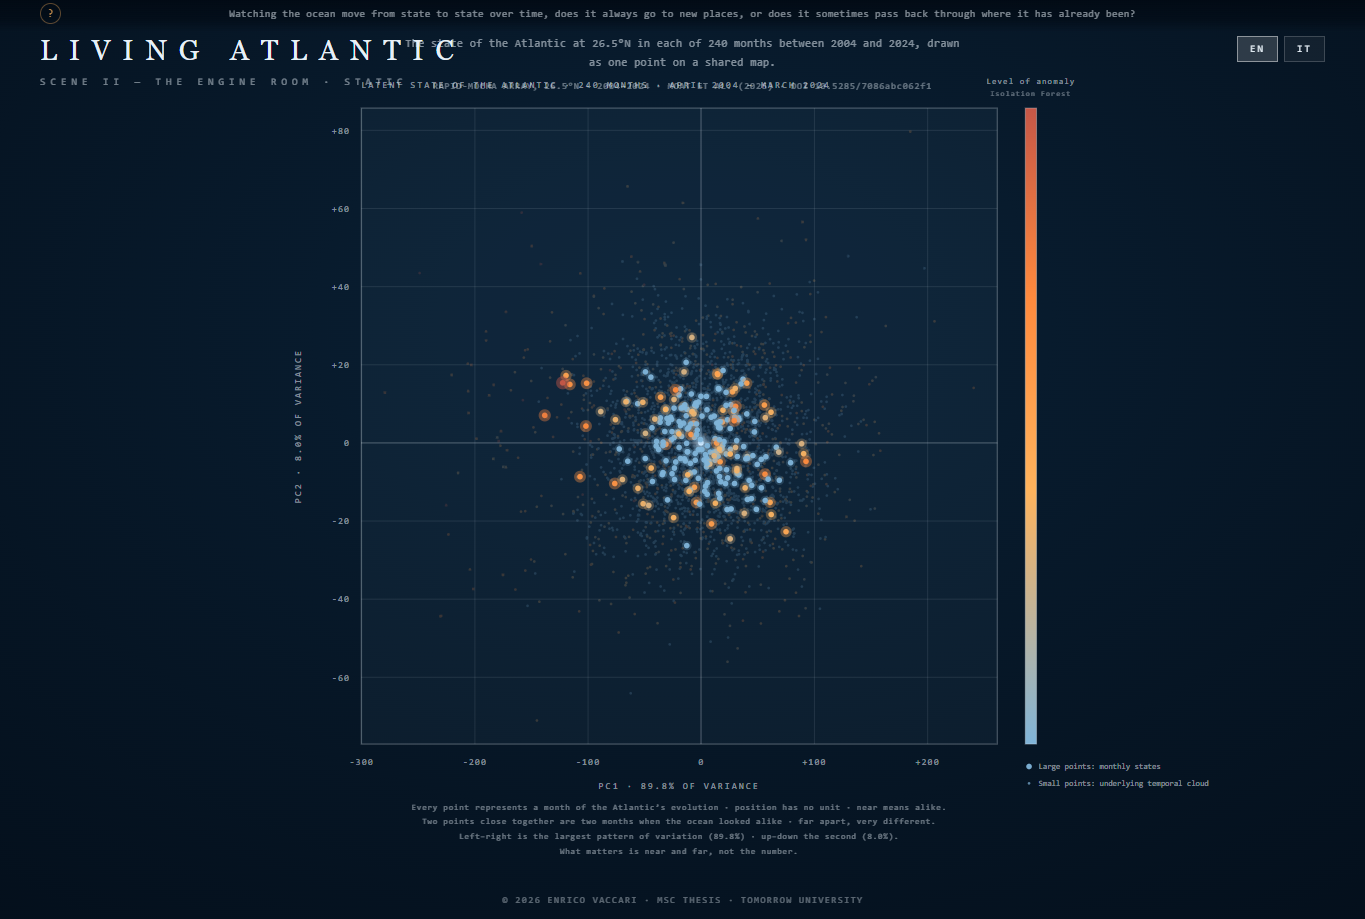
\includegraphics[width=\textwidth]{figures/viz2/viz2_theengine-static.png}
    \caption{Control (C1): the static latent-space representation.}
    \label{fig:theengine-static}
  \end{subfigure}
  \hfill
  \begin{subfigure}[t]{0.48\textwidth}
    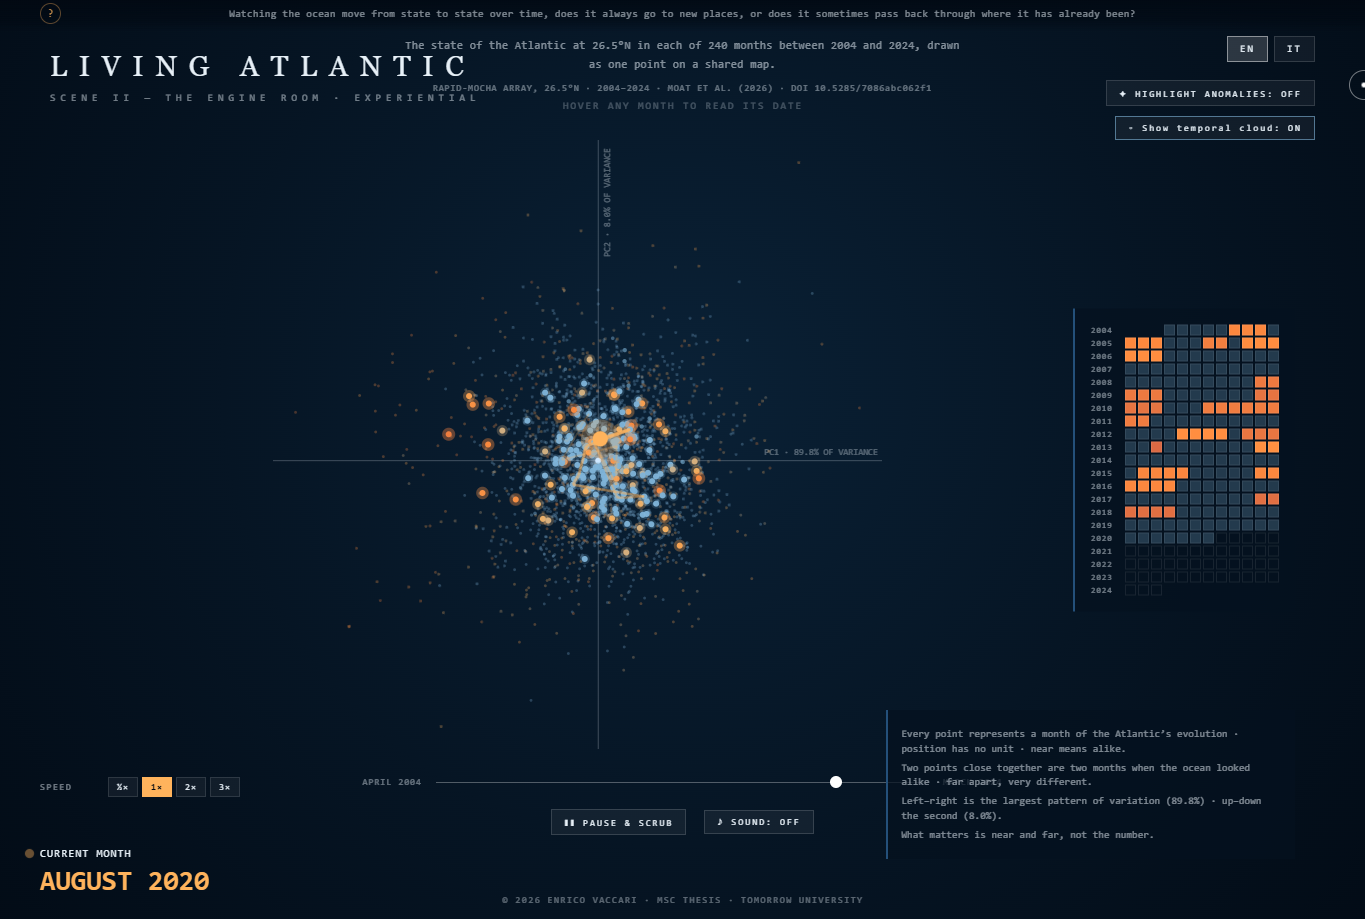
\includegraphics[width=\textwidth]{figures/viz2/viz2_theengine-experiential.png}
    \caption{Experiential (C2+C3): the evolving trajectory through latent space.}
    \label{fig:theengine-experiential}
  \end{subfigure}

  \caption[The two conditions of Scene~II]{The two administered conditions of
  Scene~II, generated from the same data bundle through the same reconstruction
  function. The static condition presents the latent structure as a fixed
  configuration, while the experiential condition reveals its temporal
  evolution.}

  \label{fig:theengine-conditions}
\end{figure}